% -*- coding: utf-8 -*-

% Relazione implementazione di un dimeostratore di teoremi mediante
% risoluzione ordinata per clausole nella logica del primo ordine
% senza uguaglianza o altri simboli interpretati
%
% Algoritmo del Ciclo della Clausola Data versione à la Otter, à la E
% senza ordinament, con ordinamento lessicografico, multiinsieme o di Knuth-Bendix
% con precedenze e pesi specificati dall'utente o in alternativa preso standard deciso
% da me (specificato nella classe Ordering)
% 


\documentclass[a4paper,11pt]{article} %{report} %{article}
\usepackage[italian]{babel} % per scrivere in italiano
\usepackage[utf8]{inputenc} % per usare lettere accentate direttamente ne .tex
\usepackage{amssymb, amsmath} % per simboli e ambienti matematici
\usepackage{amsthm}
%\usepackage{fourier} % per font utopia
\usepackage{listings} % pacchetto per codice sorgente
\usepackage{verbatim}   % useful for program listings
\usepackage{hyperref}
\usepackage{fancyhdr}
\usepackage{fancyvrb}
\usepackage{color}
\usepackage[svgnames]{xcolor}
\usepackage{url}
\usepackage{graphicx}
\usepackage{booktabs}
\usepackage{multirow}
\usepackage{siunitx}
\usepackage{caption}
\captionsetup{font=small}
\sisetup{output-decimal-marker={,}}
\usepackage{cancel}

\pagestyle{plain}

\newcommand{\sintassi}{\texttt}
\newcommand{\file}{\texttt}
\newcommand{\package}{\textbf}
\newcommand{\com}{\texttt}
\newcommand{\classe}{\textsf}
\newcommand{\metodo}{\texttt}
\newcommand{\campo}{\texttt}
\newcommand{\cod}{\lstset{basicstyle=\ttfamily}\lstinline}

\DefineVerbatimEnvironment{shell}{Verbatim}{gobble=0}

\newenvironment{myfigure}[2]
  {\newcommand{\didascalia}{\caption{#1}}%
   \newcommand{\etichetta}{\label{#2}}%
   \begin{figure}[h!]\centering}
  {\didascalia\etichetta\end{figure}}

\lstnewenvironment{codice}%
  {\lstset{language=mylang}}
  {}

\lstnewenvironment{dotgraph}%
  {\lstset{language=dot}}
  {}
  
\lstnewenvironment{tptpcod}%
  {\lstset{language=tptp}}
  {}

% DEFINIZIONE DI UNO PSEUDO LINGUAGGIO
\lstdefinelanguage{mylang}{ 
  basicstyle=\scriptsize\ttfamily,%
  keywords=[1]{const,prec,weightVars,weights,sos,clauses},keywordstyle=[1]\bfseries\sffamily,%
  keywords=[2]{int,void,String,boolean,null,Object}, keywordstyle=[2]\itshape\bfseries,%
  keywords=[3]{false,true}, keywordstyle=[3]\bfseries,%
  comment=[l]{//}, morecomment=[s]{/∗}{∗/},%
  commentstyle=\itshape\color{darkgray},%
  string=[s]{"}{"},
  stringstyle=\color{black},%
  tabsize=3,%
  escapechar=@ %
}

\lstdefinelanguage{tptp}{ 
  basicstyle=\scriptsize\ttfamily,%
  keywords=[1]{const,prec,weightVars,weights,sos,clauses},keywordstyle=[1]\bfseries\sffamily,%
  keywords=[2]{int,void,String,boolean,null,Object}, keywordstyle=[2]\itshape\bfseries,%
  keywords=[3]{false,true}, keywordstyle=[3]\bfseries,%
  comment=[l]{//}, morecomment=[s]{/∗}{∗/},%
  commentstyle=\itshape\color{darkgray},%
  string=[s]{"}{"},
  stringstyle=\color{black},%
  tabsize=3,%
  escapechar=@ %
}

\lstdefinelanguage{dot}{ 
  basicstyle=\tiny\ttfamily,%
  keywords=[1]{digraph},keywordstyle=[1]\bfseries\sffamily,%
  keywords=[2]{int,void,String,boolean,null,Object}, keywordstyle=[2]\itshape\bfseries,%
  keywords=[3]{false,true}, keywordstyle=[3]\bfseries,%
  comment=[l]{//}, morecomment=[s]{/∗}{∗/},%
  commentstyle=\itshape\color{darkgray},%
  string=[s]{"}{"},
  stringstyle=\color{black},%
  tabsize=3,%
  escapechar=@ %
}

\definecolor{MyGray}{gray}{0.75}

%\hyphenation{Ackerman} % per non sillabare la parola

%\setcounter{secnumdepth}{-2}
\setcounter{tocdepth}{2} % per inserire nell'indice fino a 2=subsection

%\evensidemargin=1cm 
\oddsidemargin=1.3cm
\headsep = 0cm
\textheight = 640pt
\textwidth = 380pt

\begin{document}

\title{Implementazione di un dimostratore di teoremi per risoluzione ordinata \\
       Ragionamento Automatico 2012-2013}
\author{Alessandro Gottoli vr352595}
%\date{}
\maketitle
%\tableofcontents % genero l'indice (doppia compilazione)

\section*{Introduzione}
L'algoritmo del ciclo della clausola data del dimostratore di teoremi
di questo progetto è stato implementato nel linguaggio di 
programmazione Java per essere eseguibile su diversi sistemi
operativi ed è stato testato su Ubuntu Linux 12.04~LTS 64~bit.
Il codice è contenuto nel package \package{thProver} e si divide in tre parti
principali: \hyperref[sec: parser]{Parser}, \hyperref[sec: interfaccia]{Interfaccia},
\hyperref[sec: ciclo]{Ciclo della clausola data}.

\section{Parser}\label{sec: parser}
Il programma accetta in ingresso file contenenti un insieme di clausole nella logica
del primo ordine in due formati differenti, quindi sono
stati implementati due parser. %perché il programma accetta in ingresso file con insieme
Uno accetta file in formato TPTP (solo sottogrammatica ``cnf''), l'altro
in un formato appositamente definito da me che ha una sintassi più simile a 
quella che troviamo in letteratura e che era stato pensato per permettere 
di definire opzioni
sull'ordinamento delle le clausole specificando precedenze (prec:) 
e pesi (weights: e weightVars), ma poi si è
deciso di aggiungere la possibilità di aggiungere tali opzioni anche all'inizio
di un file tptp anche se non previsto dalla grammatica ufficiale.
 
Questi parser si trovano nei package \package{thProver.parserTptp} e 
\package{thProver.parser} e per la generazione è stato utilizzato JavaCC, 
quindi è stata definita
la grammatica del linguaggio accettato e le azioni da fare per la costruzione
delle clausole nei file \file{GrammarTptp.jj} e \file{Grammar.jj} e le classi
java sono state create automaticamente col comando \com{javacc ``file''.jj}.

Vediamo brevemente il mio linguaggio. 
Per prima cosa dobbiamo specificare le costanti (se ci sono) scrivendo
\sintassi{const:} \emph{costante$_{1}$}\sintassi{,}
\emph{costante$_{2}$}\sintassi{,}~\ldots\sintassi{,}\emph{costante$_{n}$}.

Poi possiamo specificare le precedenze scrivendo \sintassi{prec:} 
\emph{simbolo$_{1}$} \sintassi{$>$} \emph{simbolo$_{2}$} \sintassi{$>$}~\dots
\sintassi{$>$} \emph{simbolo$_{n}$}
dove simbolo può essere un simbolo di predicato, funzione o costante. Si possono
definire precedenze parziali scrivendo
\sintassi{prec:} \emph{precedenza$_{1}$} \sintassi{;} \emph{precedenza$_{2}$}
\sintassi{;}~\dots \sintassi{;} \emph{precedenza$_{n}$}. Definire la precedenza non
è obbligatorio perché è possibile utilizzare una precedenza ``standard'' definita
nella classe ordinamento in cui \emph{predicati} $>$ \emph{funzioni} $>$ \emph{costanti}
e ogni predicato, funzione e costante è ordinata in modo da definire come
maggiore quella che viene prima nell'ordinamento lessicografico.

Si possono inoltre definire i vari pesi per utilizzarli nell'ordinamento di 
Knuth-Bendix utilizzando
\begin{itemize}
  \item{\sintassi{weightVars:} \emph{integer}} per definire il peso da dare a tutte
le variabili (così tutte avranno lo stesso peso senza doverle esplicitare)
  \item{\sintassi{weights:} \sintassi{simbolo$_{1}$ =} \emph{integer} \sintassi{;} 
\sintassi{simbolo$_{2}$ =} \emph{integer} \sintassi{;} \emph{\ldots} \sintassi{;} 
\sintassi{simbolo$_{n}$ =} \emph{integer}} per definire il peso di predicati, 
funzioni e costanti.
\end{itemize}
Se l'utente non inserisce tutti i pesi, l'ordinamento potrebbe trovarsi in 
situazioni anomale, quindi ho deciso di specificare nella classe \classe{Ordering}
il valore base per i simboli non specificati e si possono dare valori diversi 
in caso si tratti di predicati, funzioni o costanti (io ho deciso di dare valore 1).
Come per le precedenze è possibile utilizzare un peso ``standard'' definito nella
classe ordinamento in cui %tutto, di default viene pesato tutto 1 ma anche qui 
%è possibile definire un peso diverso conforme ti tratti di atomo, funzione, variabile
%o costante.
ho definito pesi per atomi, funzioni, variabili e costanti.

Adesso vediamo la sintassi di ogni clausola.
Ogni clausola è formata da uno o più letterali separati dal simbolo `\sintassi{|}'
che indica l'\emph{or}. Ogni letterale è composto da un Atomo che può essere definito
come negativo se preceduto dal simbolo `\sintassi{!}' o `\sintassi{\~}'. Ogni atomo
è poi composto da un simbolo di predicato che nella mia sintassi 
deve essere scritto con lettere maiuscole
(per essere simile alla convenzione usata in classe) 
e seguito da una eventuale lista di termini racchiusi tra `\sintassi{(}' e `\sintassi{)}'.
I termini si scrivono in minuscolo e si distinguono le funzioni (seguite dai propri
argomenti che saranno ulteriori termini racchiusi tra `\sintassi{(}' e `\sintassi{)}'),
le variabili e le costanti (che sono quelle definite all'inizio).

Adesso possiamo inserire le clausole nel seguente modo:
\vspace{-1ex}
\begin{itemize}
  \item{\sintassi{sos:} \emph{clausola$_1$} \sintassi{;} 
  \emph{clausola$_2$} \sintassi{;} \emph{\ldots} \sintassi{;} \emph{clausola$_n$}}
  per specificare le clausole da inserire nell'insieme di supporto (se usiamo questa strategia)
\vspace{-1ex}
  \item{\sintassi{clauses:} \emph{clausola$_1$} \sintassi{;} 
  \emph{clausola$_2$} \sintassi{;} \emph{\ldots} \sintassi{;} \emph{clausola$_n$}}
  per specificare le altre clausole.
\end{itemize}
\vspace{-1ex}
Anche se non si ha intenzione di utilizzare l'insieme di supporto si possono
specificare lo stesso come `sos' le clausole provenienti dalla trasformazione in
forma clausale della negazione della congettura, perché se non verrà attivata la
strategia verranno unite alle altre clausole.

Anche per il formato tptp è possibile utilizzare la strategia dell'insieme di 
supporto, infatti nella sintassi c'è un campo \emph{ruolo} e nell'insieme di
supporto inserisco quelle che hanno come ruolo \emph{``negated\_conjecture''}.

%Ecco un esempio di file di input di un esercizio fatto in classe:
%\vspace{-1ex}
%\begin{shell}
%const: a,b,c
%prec: ON>GREEN ; a>b>c
%weightVars: 1
%weights: ON = 1; GREEN = 1; a = 1; b = 1; c = 1
%sos: ~GREEN(x) | GREEN(y) | ~ON(x,y)
%clauses: ON(a,b) ; ON(b,c) ; GREEN(a) ; ~GREEN(c)
%\end{shell}
Un esempio di file di input è mostrato in Figura~\ref{fig: esempio input}
\begin{myfigure}{Esempio di file di input.}{fig: esempio input}
\begin{tabular}{c}
\begin{codice}
const: a,b,c
prec: ON>GREEN ; a>b>c
weightVars: 1
weights: ON = 1; GREEN = 1; a = 1; b = 1; c = 1
sos: ~GREEN(x) | GREEN(y) | ~ON(x,y)
clauses: ON(a,b) ; ON(b,c) ; GREEN(a) ; ~GREEN(c)
\end{codice}
\end{tabular}
\end{myfigure}


\section{Interfaccia}\label{sec: interfaccia}
L'elaborato è fornito di due interfacce: una a 
\hyperref[subsec: int. linea]{linea di comando} e una 
\hyperref[subsec: int. grafica]{grafica}.

\subsection{Interfaccia a linea di comando}\label{subsec: int. linea}
Questa interfaccia è quella predefinita e come si può vedere dall'``usage''
si possono attivare i diversi parametri specificando le diverse opzioni quando
si avvia il programma.

Per prima cosa si specifica l'input e sono disponibili due alternative:
\vspace{-1ex}
\begin{itemize}
  \item{\sintassi{-i}} indica che si vuole inserire la formula da standard input in modo iterativo
\vspace{-1ex}
  \item{\sintassi{/percorso\_del\_file/input.p}} per caricare da file
\end{itemize}
\vspace{-1ex}
\`E obbligatorio specificarne una altrimenti il programma terminerà.

Poi può specificare di utilizzare la strategia dell'insieme di supporto con 
``\sintassi{-sos}'', di default non è attivata.

Di default non si utilizza nessun ordinamento, però sono disponibili le seguenti 
opzioni per selezionarne uno:
\vspace{-1ex}
\begin{itemize}
  \item{\sintassi{-lex}} per l'ordinamento ricorsivo a cammini con status lessicografico
\vspace{-1ex}
  \item{\sintassi{-mul}} per l'ordinamento ricorsivo a cammini con status multiinsieme
\vspace{-1ex}
  \item{\sintassi{-kbo}} per l'ordinamento di Knuth-Bendix
\end{itemize}
\vspace{-1ex}
Una volta scelto l'ordinamento il programma utilizzerà di default quello 
``standard''definito da me nel programma
(utile se non sono state specificate le precedenze o i pesi nell'input),
ma digitando ``\sintassi{-usP}'' si possono utilizzare le precedenze e i pesi definiti 
nell'input.

Il ciclo della clausola data ha due versioni che differiscono principalmente
sull'insieme di clausole da mantenere interridotto. L'elaborato le implementa
entrambe ed utilizza di default la versione \emph{à~la~Otter}, mentre è possibile
selezionare la versione \emph{à~la~E} con il parametro \sintassi{-E}.

\`E stata inoltre aggiunta l'opzione ``\sintassi{-limit}\emph{n\_secondi}'' che permette 
di fermare la computazione quando è passato il tempo indicato.


%\subsection{Interfaccia grafica}\label{subsec: int. grafica} 
\begin{subsection}{Interfaccia grafica}\label{subsec: int. grafica}
Questa interfaccia è attivabile specificando l'opzione ``\sintassi{-gui}'' quando si
lancia il programma e verrà visualizzata una finestra in cui poter inserire
direttamente l'input oppure selezionare un file. Le altre opzioni sono bloccate
in modo da rendere selezionabili sono quelle applicabili dopo aver fatto il
parsing. La cosa carina è che si possono fare risoluzioni diverse sullo stesso 
input facendo solo una volta la fase di parsing.
\end{subsection}

In entrambe le interfacce c'è la possibilità (se l'input risulta insoddisfacibile)
di salvare un file con sintassi `dot' in cui è specificato il grafo diretto
della prova di refutazione indicando le clausole e le regole di inferenza 
utilizzate ad ogni passo (compresa la sostituzione).
Per esempio %il grafo della prova dell'esempio in Figura~\ref{fig: esempio input}
%ottenuto 
con Otter e ordinamento lessicografico definito dall'utente %è visualizzabile
si ottiene il sorgente in Figura~\ref{fig: src grafo prova} come prova di insoddisfacibilità
della formula dell'esempio definito in precedenza.

Inoltre se sulla macchina è installato `dot' (su linux si tratta del pacchetto
\emph{graphviz}) è possibile esportare anche l'immagine del grafo vero e proprio in formato
jpg, ps e pdf (esempi di questi file si trovano nella directory dei problemi 
testati con specificate anche le opzioni del programma che ha permesso di trovare
quella prova).
L'immagine ottenuta dal sorgente in Figura~\ref{fig: src grafo prova} si trova in 
Figura~\ref{fig: grafo prova}.
\vspace{-4ex}
\begin{myfigure}{File sorgente per `dot' del grafo della prova.}{fig: src grafo prova}
%\begin{tabular}{c}
\centering
\begin{dotgraph}
digraph {
	nodesep="1.5"; ranksep=2;
	node [shape=plaintext];
	edge [color=gray];
	"GREEN(c)" -> "[]" 
		[labelfontcolor=black,labelfontsize="12",headlabel="Ordered Resolution\n{ }",labeldistance="6"];
	"~GREEN(b) | GREEN(c)" -> "GREEN(c)" 
		[labelfontcolor=black,labelfontsize="12",headlabel="Ordered Resolution\n{ }",labeldistance="6"];
	"~GREEN(x_0) | GREEN(y_0) | ~ON(x_0,y_0)" -> "~GREEN(b) | GREEN(c)" 
		[labelfontcolor=black,labelfontsize="12",headlabel="Ordered Resolution\n{ x_0 <- b, y_0 <- c }",labeldistance="6"];
	"ON(b,c)" -> "~GREEN(b) | GREEN(c)" ;
	"GREEN(b)" -> "GREEN(c)" ;
	"GREEN(a)" -> "GREEN(b)" 
		[labelfontcolor=black,labelfontsize="12",headlabel="Clausal Simplification\n{ }",labeldistance="6"];
	"~GREEN(a) | GREEN(b)" -> "GREEN(b)" ;
	"~GREEN(x_0) | GREEN(y_0) | ~ON(x_0,y_0)" -> "~GREEN(a) | GREEN(b)" 
		[labelfontcolor=black,labelfontsize="12",headlabel="Ordered Resolution\n{ x_0 <- a, y_0 <- b }",labeldistance="6"];
	"ON(a,b)" -> "~GREEN(a) | GREEN(b)" ;
	"~GREEN(c)" -> "[]" ;
}
\end{dotgraph}
%\end{tabular}
\end{myfigure}
\vspace{-5ex}
\begin{myfigure}{Grafo della prova.}{fig: grafo prova}
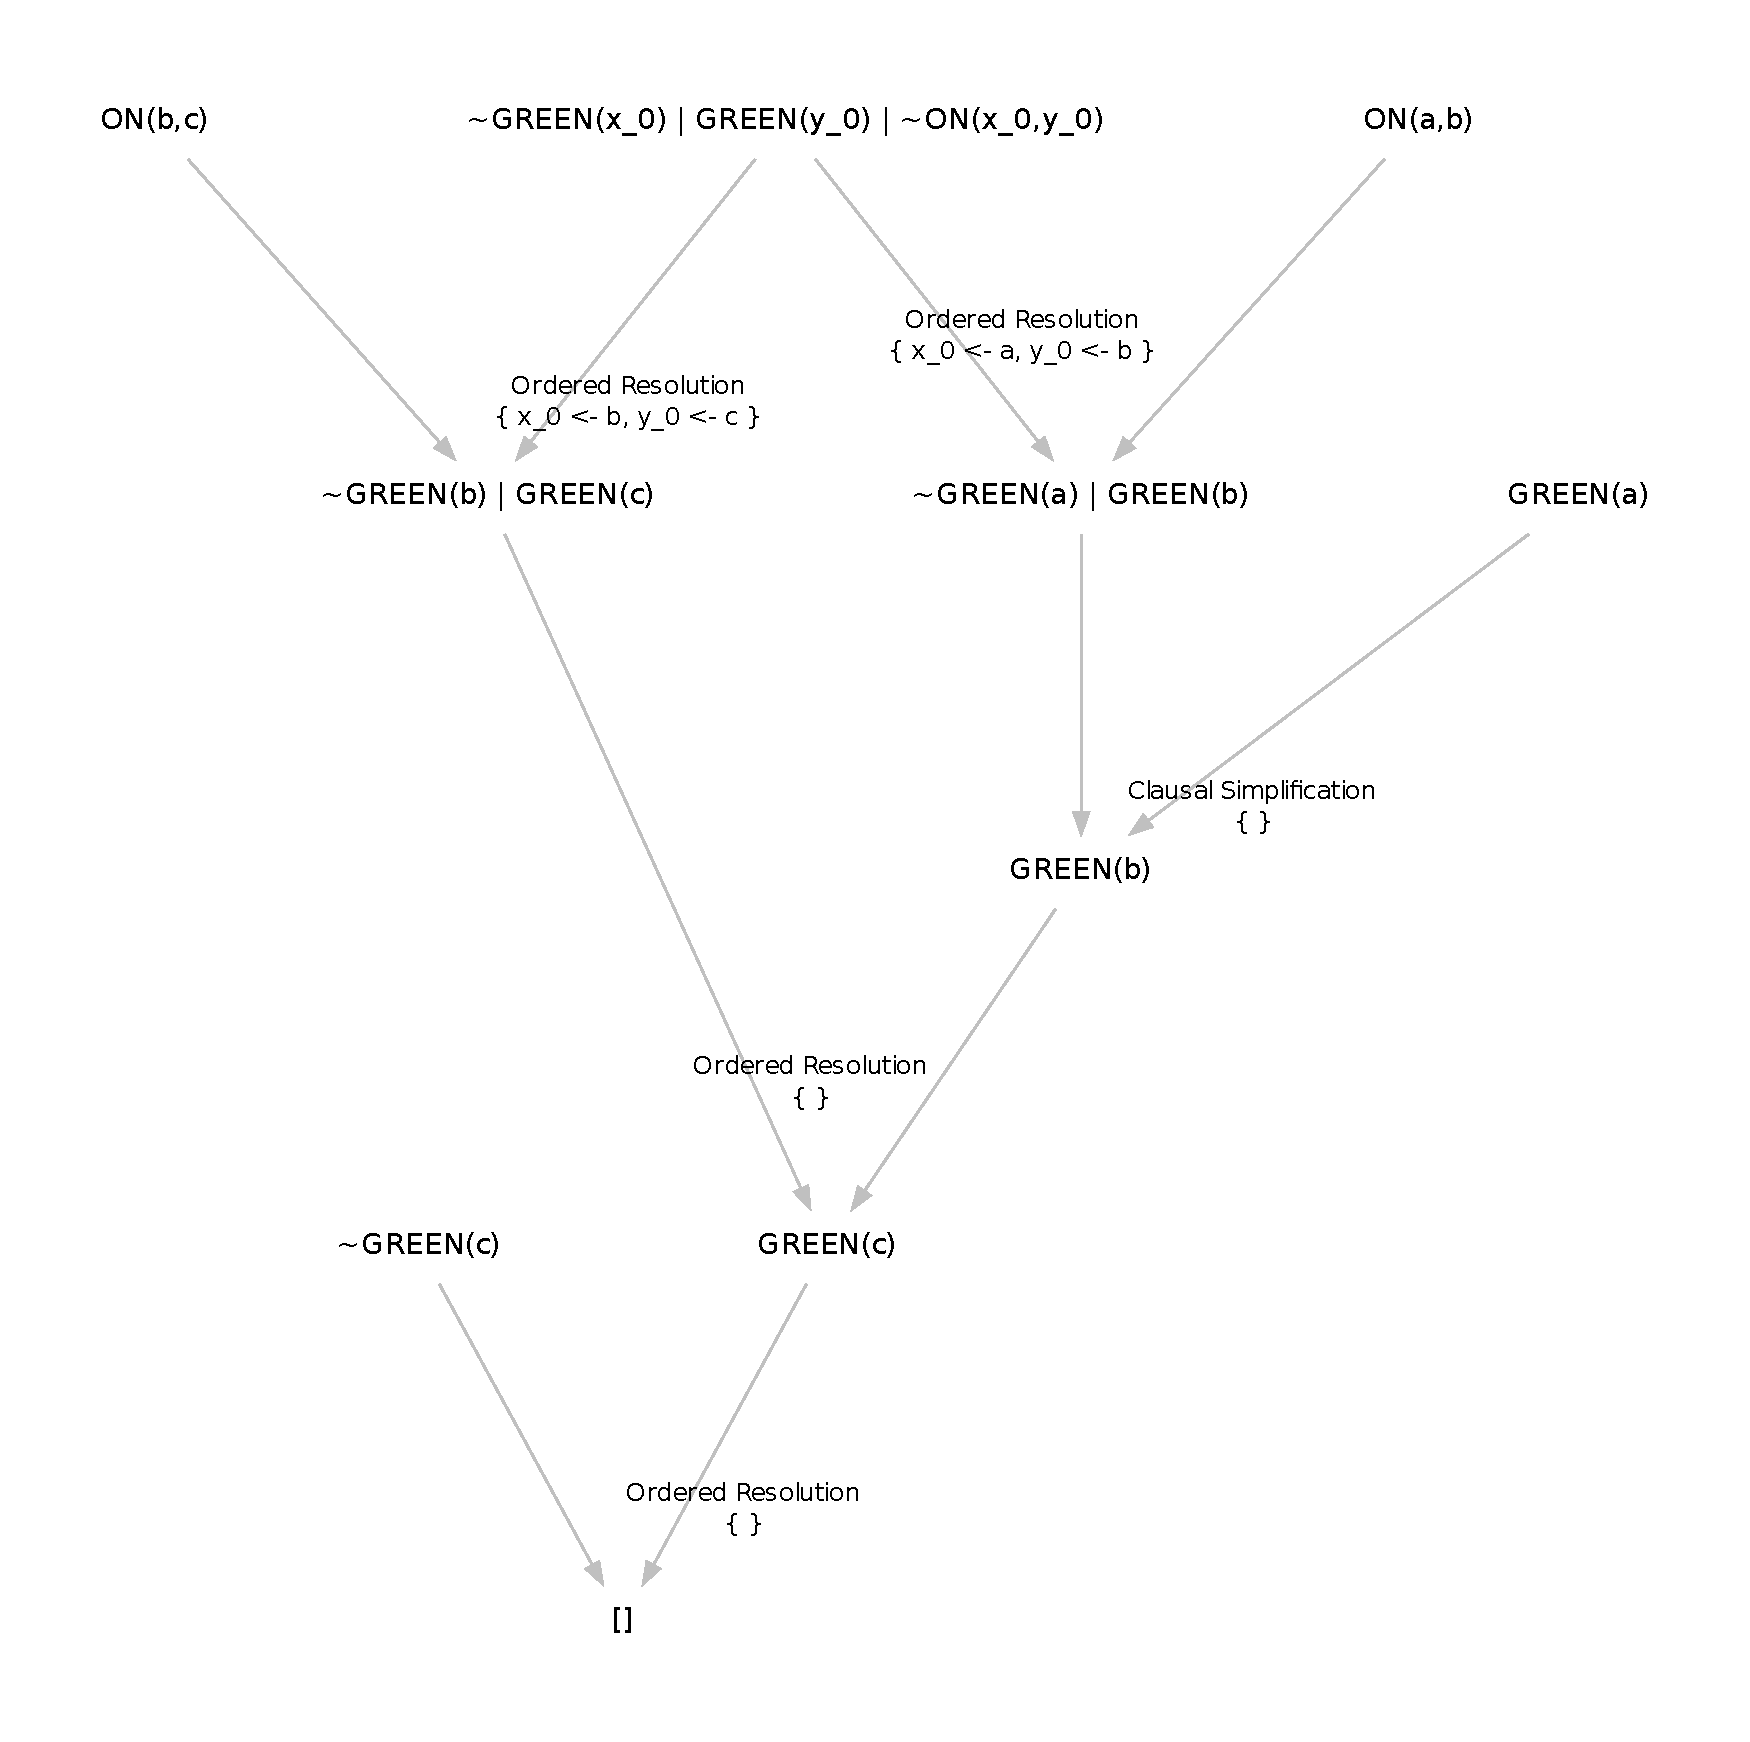
\includegraphics[width=.90\columnwidth]{blocks-Otter-lex-usP}
\end{myfigure}

\section{Ciclo della clausola data}\label{sec: ciclo}
Adesso vediamo il codice che esegue la computazione vera e propria della
suddisfacibilità della formula data in input.

Il main dopo aver processato i parametri dati dall'utente ed aver letto l'input
esegue il parsing che istanzia un oggetto \classe{CNFFormula} che
conterrà tutti i dati relativi all'input. Esso contiene diverse \classe{HashMap} 
in cui salvo atomi e termini così creo una sola istanza dello stesso oggetto
che verrà condivisa, 
poi ce nè una
che mappa simbolo con la propria arietà per controllare in fase di parsing
che non vengano passati un numero diverso di argomenti allo stesso simbolo. 
Ci sono poi altre
strutture per le precedenze e i pesi. 
Quando si processano le variabili di clausole diverse bisogna intenderle disgiunte
anche se hanno lo stesso simbolo, allora ho deciso di rinominarle alla creazione 
assegnandogli come nuovo simbolo univoco 
\sintassi{simbolo\_indiceclausola} così non c'è problema di rinominarle ad ogni
risoluzione. In caso di risoluzione in cui la nuova clausola dovesse contenere
\sintassi{x\_1} e \sintassi{x\_2} contemporaneamente, bisogna stare attenti a non confonderle
rinominandole entrambe con l'indice della nuova clausola, così è stato implementato
un metodo che in caso di ``simbolo originale'' uguale ma indice diverso
si otterrà per esempio \sintassi{x\_3} e \sintassi{x'\_3} disambiguando le variabili
con ``\sintassi{'}''.
% e in caso si dovesse incontrare una clausola che dovrebbe contenere
% x_1 e x_2 senza unificarle è stato aggiunto un metodo che rende le variabili
% x_3 e x'_3 tendendo sempre la numerazione ma disambiguandole con il ``'''.

Subito dopo genera un oggetto \classe{Ordering} che implementa i tre ordinamenti
e setta quello selezionato dall'utente. Siccome nelle api java non c'è una classe che implementi
i multiinsiemi è stata implementata in \classe{MultiSet} utilizzando 
un'\classe{HashMap$<$Object, Integer$>$} in cui salvare l'oggetto con il conto del
numero di occorrenze. Per poter adottare questa implementazione si è resa 
necessaria l'implementazione dei metodi \metodo{equals} e \metodo{hashCode}
altrimenti istanze diverse rappresentanti lo stesso elemento sarebbero state 
mappate in oggetti differenti avendo avuto di default i metodi ereditati da \classe{Object}. 

Adesso è tutto pronto per verificare l'insoddisfacbilità della formula inserita.
Il ciclo della clausola data %vero e proprio 
è implementato nella classe
\classe{GivenClauseProver} nel metodo \metodo{satisfiable} che prende in ingresso
un oggetto \classe{CNFFormula} che contiene tutte le clausole generate nella
fase di parsing, costruisce le liste ``\campo{To\_Select}'' e ``\campo{Selected}'' ed esegue il
ciclo while fino a che ``\campo{To\_Select}'' risulta vuoto o trova la clausola vuota.
Ho scelto di implementare l'insieme delle clausole ``\campo{To\_Select}'' come una
\classe{PriorityQueue} in cui scelgo la clausola data con il minor numero
di simboli per avere un'ordinamento \emph{equo} (in caso di valore uguale
sceglierò la clausola con indice minore), mentre ``Selected'' è un
semplice ArrayList perché devo scorrerlo tutto ogni volta per fare risoluzione.

Durante il ciclo verranno utilizzate le regole del nostro insieme di inferenza
che si trovano in \classe{InferenceSystem} che
implementa appunto il sistema di inferenza.
La classe contiene anche il metodo \metodo{mgu} che
aggiorna una sostituzione in modo da trovare l'\emph{unificatore più generale} 
tra due letterali nelle regole di inferenza. Siccome nella sussunzione e nella
semplificazione clausale la sostituzione va applicata solo da un lato, è
stato aggiunto un flag booleano per imporre questa restrizione in fase di unificazione. 
Per le sostituzioni sopra citate viene definita una classe apposita \classe{Substitution}
con all'interno una \classe{HashMap}$<$\classe{Variable}, \classe{Term}$>$ che
rende veloce la ricerca del termine da sostituire alla variabile e sono inclusi
anche i vari metodi per controllare che sia idempotente.
% Questi metodi utilizzano i ``veri''
%metodi degli oggetti \classe{Clause}.

Il maggior lavoro per trovare una soluzione implementativa efficiente è stato
fatto proprio in \classe{Clause} (le clausole), perché la maggior parte dei metodi sono applicati
proprio a loro. Aprendo la classe si nota subito che i letterali che compongono la clausola
sono inseriti
sia in un \classe{Set} \cod{literals} sia in due liste \cod{posLits} e \cod{negLits} (essendo
liste di puntatori non si consuma eccessiva memoria). Questo mi permette di 
lavorare solo su letterali con il segno che interessa per la tale regola senza
il bisogno di fare due cicli for annidati che confrontano anche elementi che
sappiamo a priori non essere compatibili. 

Siccome le clausole sono 
``immodificabili'' l'approccio che ho pensato è che tutti i metodi che 
possono impiegare parecchio tempo a calcolare un risultato che alle successive 
chiamate non cambia, devono salvare il risultato per usi futuri.
I dati relativi agli ordinamenti ne sono un esempio, infatti posso calcolare
i letterali massimali solo la prima volta dato quell'ordinamento e salvandoli in
\cod{maximalLiterals} riutilizzarli senza ricalcolarli ad ogni inferenza.
Come i letterali anche questi li salvo in \cod{posMaximalLits} e 
\cod{negMaximalLits} per guadagnare confronti inutili.

Altri esempi sono \cod{numSymbs} che contiene il numero di simboli che sarebbe 
necessario ricalcolare ricorsivamente ad ogni iterazione del ciclo della clausola data
per ordinare la coda di priorità (questo vale anche per i sottotermini che 
vengono condivisi che calcolano il loro valore solo la prima volta)
e \cod{stringa} che contiene la rappresentazione della clausola.
Questi ultimi due sono utili anche se facciamo partire più volte
la prova sullo stesso input (come può avvienire tranquillamente nella GUI), solo la prima mi 
calcolerà i risultati rendendo più veloci le successive.

Poi ci sono dei campi aggiuntivi \cod{parents}, \cod{substitutionFrom} e \cod{rule}
che ci permettono di tenere traccia dell'albero di derivazione e di costruire il
grafo.

Altra scelta implementativa è stata l'implementazione della sussunzione, infatti
in \classe{Clause} ci sono due metodi per la sussunzione. \metodo{subsumes} è la
mia versione che implementa la sia la \emph{sussunzione propria} sia quella 
\emph{di varianti} confrontando delle liste con lo stesso simbolo di predicato e
stesso segno e cercando di unificare i letterali tra le due clausole.
\metodo{subsumesChangLee} invece è l'implementazione descritta nel Chang-Lee
a pag.~95 e prevede di calcolare vari risolveni tra le clausole.
A livello di test la mia versione risulta più venoce perché richiede solo di trovare
gli \metodo{mgu} e non fare tutta la risoluzione. Inoltre mettendo la condizione
aggiuntiva sul numero di letterali nella sussunzione propria 
($|$C$|$~$<$~$|$D$|$) e il numero di indice nella di varianti (in(C)~$<$~id(D))
la mia sussume meno clausole rispetto quella del Chang-Lee. Un esempio è:
C~=~\cod{P(x) | P(f(y))} e D~=~\cod{P(f(z))} che per la versione Chang-Lee risulta
C~sussume~D, mentre con la mia no. Questa differenza però non ha ripercussioni
sul risultato finale. Si può provare la seconda versione inserendo
il parametro aggiuntivo \sintassi{-changlee} all'avvio del programma ed è 
disponibile solo nell'interfaccia a riga di comando perché serve solo per test.


\section{Risultati degli esperimenti}\label{sec: esperimenti}
Nella maggior parte dei casi le procedure con ordinamento generano meno clausole
rispetto a non utilizzarli e nei casi in cui si arriva a soluzione 
per clausola vuota o per insieme ``\campo{To\_Select}'' vuoto sono più veloci.
%Ovviamente trattandosi di un problema semidecidibile c'è anche il caso in cui 
%si diverge e quindi non si avrà alcun vantaggio.

Anche l'utilizzo dell'insieme di supporto riduce di molto il tempo di esecuzione
della procedura%, però su alcuni esempi tptp (mettere nomi\ldots) è stato 
%riscontrato che abbinato ad ordinamenti porta
%problemi insoddisfacibili a dare come risposta soddisfacibile
%per ``\campo{To\_Select}'' vuoto.
 e spesso risulta migliore anche rispetto agli ordinamenti,
ma questo probabilmente perché gli ordinamenti non sono stati scelti ad hoc per il
problema in esame. 

Si è provato ad unire ordinamenti e strategia dell'insieme di suporto per vedere
se si ottenevano ulteriori miglioramenti, ma dagli esperimenti si è notato che 
%utilizzare la strategia di supporto
%con la risoluzione ordinata comporta la perdita della completezza refutazionale.
non sono compatibili, infatti molto spesso da risultato errato.  
%Questo
%probabilmente è dovuto al fatto che non sia la congettura negata a rendere 
%insoddisfacibile l'insieme di clausole. Quindi se l'insieme di clausole 
%S~=~$<$T~$\uplus$~sos$>$ risulta 
%soddisfacibile, il motivo è che T non è consistente.
Un esempio è il file ``\file{vr352595/Problemi/tptp.file/ALG002-1.p}'' che con Otter e
sos da come output:
\scriptsize
\vspace{-1ex}
\begin{shell}
/* info */
14 clauses from parsing, 
2780 clauses generated, 
1651 clauses deleted, 
963 clauses in To_Select, 
160 clauses in Selected, 
in 6 sec. and 583 millisec..
response: UNSATISFIABLE.
\end{shell}
\normalsize
Mentre con Otter, sos e ordinamento Knuth-Bendix predefinito da:
\scriptsize
\vspace{-1ex}
\begin{shell}
/* info */
14 clauses from parsing, 
0 clauses generated, 
0 clauses deleted, 
0 clauses in To_Select, 
14 clauses in Selected, 
in 5 millisec..
response: SATISFIABLE.
\end{shell}
\normalsize
%Infatti analizzando la prova di refutazione in 
%%``\file{vr352595/Problemi/tptp.file/risultati/ALG002-1.p/ALG002-1-Otter-sos.pdf}''
%``\file{vr352595/Problemi/tptp.file/}
%\file{risultati/ALG002-1.p/ALG002-1-Otter-sos.pdf}''
%si nota che tutto ha inizio con il risolvente tra
%\begin{tptpcod}
%cnf(product_and_inverse,axiom,
%    ( greater_than_0(X)
%    | product(X,X,additive_identity)
%    | greater_than_0(additive_inverse(X)) )).
%
%cnf(prove_a_inverse_greater_than_0,negated_conjecture,
%    ( ~ greater_than_0(multiplicative_inverse(a)) )).
%\end{tptpcod}
%
Infatti per fare risoluzione bisogna per forza %usare 
%``\cod{greater_than_0(X)} \cod{|} \cod{product(X,X,additive_identity)} \cod{|} 
%\cod{greater_than_0(additive_inverse(X))}'' o 
%``\cod{~ product(Y,Z,X)} \cod{|} \cod{~ greater_than_0(Y)} \cod{|} 
%\cod{~ greater_than_0(Z)} \cod{|} \cod{greater_than_0(X)}''
%e 
unificare %con ``\cod{~ greater_than_0(multiplicative_inverse(a))}''
%che è possibile solo 
usando
\cod{greater_than_0(X)} %e \cod{~greater_than_0(multiplicative_inverse(a))}
che però con kbo non risulta tra i letterali massimali.
%infatti \cod{greater_than_0(additive_inverse(X))} e 
%\cod{~ product(Y,Z,X)} risultano maggiori nelle rispettive clausole.
Addirittura se proviamo con ordinamento lessicografico o multiinsieme 
la computazione sembra divergere.
Si possono vedere questi risultati in alcuni esperimenti riportati
in Tabella~\ref{tab: tptp otter}. Per questione di spazio
è stato espresso con \textsf{T} il numero finale di clausole in 
``\campo{To\_Select}'',
\textsf{S} il numero finale di clausole in ``\campo{Selected}'',
\textsf{G} il numero finale di clausole generate e
\textsf{D} il numero finale di clausole eliminate..

Sono state confrontate anche la versione à la Otter con quella à la E e
come ci si aspettava il numero di clausole generate dalla versione à la E
sono maggiori, ma nonostante questo la maggior parte dei casi
è risultata più veloce.
Alcuni confronti tra le versioni con e senza l'utilizzo degli ordinamenti
o dell'insieme di supporto
si trovano nella Tabella~\ref{tab: tptp otter} per à la Otter
e nella Tabella~\ref{tab: tptp E}.

%%%%%%%%%%%%%%%%%%%%%%%%%%%%%%%%%%
Ho provato anche un'approccio diverso del ciclo della clausola data.
Mentre nell'originale si fa risoluzione tra la
%ogni clausola risolvente deve avere come padre la clausola
data e una clausola in ``\campo{Selected}'' 
e si calcolano i fattori della clausola data
per poi aggiungere tutte le nuove clausole
in ``\campo{To\_Select}''; io ho provato a calcolare tutti i risolventi tra
la clausola data e le clausole in ``\campo{Selected}'' compresi quelli calcolati 
sui fattori di esse e aggiungendo solo questi risolventi in ``\campo{To\_Select}''.
Il risultato della prova di soddisfacibilità è lo stesso, anche se il mio esperimento
risulta più lento. Se si desidera è possibile provarlo inserendo
il parametro aggiuntivo \sintassi{-vAll} all'avvio del programma ed è 
disponibile solo nell'interfaccia a riga di comando perché serve solo per test.
Di default comunque verrà utilizzata la versione corretta come da specifica.
I rilevamenti effettuati sono stati riportati in Tabella~\ref{tab: sussunzione + vAll}
nella quale è stato inserito anche il confronto tra i due tipi di sussunzione
menzionati precedentemente.
%%%%%%%%%%%%%%%%%%%%%%%%%%%%%%%%%%

Alcuni esercizi fatti in classe sono stati risolti con l'elaborato e i
risultati si trovano in Tabella~\ref{tab: esempi in classe}.

Nelle tabelle sono stati riportati solo i risultati più interessanti, 
tutti i rilevamenti effettuati si possono trovare nella cartella \file{risultati}
relativa ad ogni problema.

%% TABELLA RISULTATI %%
%Legenda
%Ris. risultato dell’esecuzione
%T numero finale di clausole in To_Select
%S numero finale di clausole in Selected
%G numero finale di clausole generate
%D numero finale di clausole eliminate
%Tempo tempo di esecuzione 

%%%%%%%%%%%%%%%% incompatibilità sos + ordinamento (esempi solo kbo)
%\begin{table}
%\centering
%\small
%\begin{tabular}{lllS[table-format=5.0]S[table-format=5.0]S[table-format=5.0]S[table-format=5.0]l}
%\toprule
% & \textbf{à la Otter} & & & & & & \\
%File & \textsf{Opzioni} & {Risposta} & {G} & {D} & {T} & {S} & tempo \\
%\midrule\midrule
%
%\multirow{2}*{\file{ALG002-1.p}} 
%                    &  & \emph{SAT} & 31959 & 20178 & 10973 & 803 & \emph{timeout} \\
%\cmidrule(l){2-8}
%                    & kbo & \emph{SAT} & 46897 & 37897 & 28 & 9395 & \emph{timeout} \\
%\cmidrule(l){2-8}
%                    & sos & UNSAT & 2780 & 1651 & 963 & 161 & 6 sec. 141 millisec. \\
%\cmidrule(l){2-8}
%                    & sos + kbo & SAT & 0 & 0 & 0 & 14 & 5 millisec. \\
%\midrule\midrule
%
%\multirow{2}*{\file{COL123-2.p}} 
%                    &  & \emph{SAT} & 12892 & 2869 & 8900 & 1104 & \emph{timeout} \\
%\cmidrule(l){2-8}
%                    & kbo & \emph{SAT} & 34853 & 26975 & 6932 & 954 & \emph{timeout} \\
%\cmidrule(l){2-8}
%                    & sos & UNSAT & 28691 & 19587 & 7026 & 2070 & 4 min. 24 sec. \\
%\cmidrule(l){2-8}
%                    & sos + kbo & SAT & 501 & 214 & 174 & 120 & 1 sec. 645 millisec. \\
%\midrule\midrule
%
%\multirow{2}*{\file{COM001-1.p}} 
%                    &  & UNSAT & 13364 & 12170 & 903 & 197 & 6 sec. 336 millisec. \\
%\cmidrule(l){2-8}
%                    & kbo & UNSAT & 1071 & 874 & 114 & 53 & 1 sec. 213 millisec. \\
%\cmidrule(l){2-8}
%                    & sos & UNSAT & 48 & 5 & 25 & 28 & 156 millisec. \\
%\cmidrule(l){2-8}
%                    & sos + kbo & \emph{SAT} & 20665 & 13112 & 6377 & 1187 & \emph{timeout} \\
%\midrule\midrule
%
%\multirow{2}*{\file{PLA001-1.p}} 
%                    &  & UNSAT & 272 & 66 & 145 & 76 & 1 sec. 139 millisec. \\
%\cmidrule(l){2-8}
%                    & kbo & UNSAT & 216 & 104 & 44 & 83 & 550 millisec. \\
%\cmidrule(l){2-8}
%                    & sos & UNSAT & 117 & 49 & 31 & 52 & 346 millisec. \\
%\cmidrule(l){2-8}
%                    & sos + kbo & UNSAT & 538 & 292 & 121 & 140 & 1 sec. 697 millisec. \\
%\midrule\midrule
%
%\multirow{2}*{\file{PLA003-1.p}} 
%                    &  & UNSAT & 78 & 40 & 16 & 31 & 231 millisec. \\
%\cmidrule(l){2-8}
%                    & kbo & UNSAT & 737 & 673 & 1 & 54 & 1 sec. 158 millisec. \\
%\cmidrule(l){2-8}
%                    & sos & UNSAT & 55 & 31 & 2 & 31 & 155 millisec. \\
%\cmidrule(l){2-8}
%                    & sos + kbo & SAT & 1 & 1 & 0 & 11 & 10 millisec. \\
%\bottomrule
%\end{tabular}
%\caption{Rilevamenti ciclo à la Otter applicato a file tptp.}
%\label{tab: tptp otter}
%\end{table}


%%%%%%%%%%%%%%%% à la Otter
\begin{table}
\centering
\scriptsize
\begin{tabular}{lllS[table-format=5.0]S[table-format=5.0]S[table-format=5.0]S[table-format=5.0]l}
\toprule
 & \textbf{à la Otter} & & & & & & \\
%\multicolumn{1}{c}{File} & tipo & Ris & T & S & G & D & tempo \\
File & \textsf{Opzioni} & {Risposta} & {G} & {D} & {T} & {S} & tempo \\
\midrule%\midrule

\multirow{2}*{\file{ALG002-1.p}} 
                    &  & \emph{SAT} & 31959 & 20178 & 10973 & 803 & \emph{timeout} \\
\cmidrule(l){2-8}
                    & \com{-lex} & \emph{SAT} & 15229 & 6963 & 7595 & 685 & \emph{timeout} \\
\cmidrule(l){2-8}
                    & \com{-mul} & \emph{SAT} & 15156 & 6905 & 7593 & 672 & \emph{timeout} \\
\cmidrule(l){2-8}
                    & \com{-kbo} & \emph{SAT} & 46897 & 37897 & 28 & 9395 & \emph{timeout} \\
\cmidrule(l){2-8}
                    & \com{-sos} & UNSAT & 2780 & 1651 & 963 & 161 & 6 sec. 141 millisec. \\
\cmidrule(l){2-8}
                    & \com{-sos -kbo} & \cancel{SAT} & 0 & 0 & 0 & 14 & 5 millisec. \\
%\cmidrule(l){2-8}
\midrule%\midrule

\multirow{2}*{\file{COL123-2.p}} 
                    &  & \emph{SAT} & 12892 & 2869 & 8900 & 1104 & \emph{timeout} \\
\cmidrule(l){2-8}
                    & \com{-lex} & UNSAT & 4080 & 257 & 3316 & 490 & 35 sec. 459 millisec. \\
\cmidrule(l){2-8}
                    & \com{-mul} & UNSAT & 3743 & 2627 & 911 & 212 & 8 sec. 553 millisec. \\
\cmidrule(l){2-8}
                    & \com{-kbo} & \emph{SAT} & 34853 & 26975 & 6932 & 954 & \emph{timeout} \\
\cmidrule(l){2-8}
                    & \com{-sos} & UNSAT & 28691 & 19587 & 7026 & 2070 & 4 min. 24 sec. \\
\cmidrule(l){2-8}
                    & \com{-sos -kbo} & \cancel{SAT} & 501 & 214 & 174 & 120 & 1 sec. 645 millisec. \\
%\cmidrule(l){2-8}
\midrule%\midrule

\multirow{2}*{\file{COM001-1.p}} 
                    &  & UNSAT & 13364 & 12170 & 903 & 197 & 6 sec. 336 millisec. \\
\cmidrule(l){2-8}
                    & \com{-lex} & UNSAT & 1071 & 874 & 114 & 53 & 1 sec. 131 millisec. \\
\cmidrule(l){2-8}
                    & \com{-mul} & UNSAT & 883 & 705 & 103 & 50 & 1 sec. 18 millisec. \\
\cmidrule(l){2-8}
                    & \com{-kbo} & UNSAT & 1071 & 874 & 114 & 53 & 1 sec. 213 millisec. \\
\cmidrule(l){2-8}
                    & \com{-sos} & UNSAT & 48 & 5 & 25 & 28 & 156 millisec. \\
\cmidrule(l){2-8}
                    & \com{-sos -kbo} & \emph{SAT} & 20665 & 13112 & 6377 & 1187 & \emph{timeout} \\
%\cmidrule(l){2-8}
\midrule%\midrule

\multirow{2}*{\file{PLA001-1.p}} 
                    &  & UNSAT & 272 & 66 & 145 & 76 & 1 sec. 139 millisec. \\
\cmidrule(l){2-8}
                    & \com{-lex} & UNSAT & 216 & 104 & 44 & 83 & 562 millisec. \\
\cmidrule(l){2-8}
                    & \com{-mul} & UNSAT & 213 & 101 & 44 & 83 & 583 millisec. \\
\cmidrule(l){2-8}
                    & \com{-kbo} & UNSAT & 216 & 104 & 44 & 83 & 550 millisec. \\
\cmidrule(l){2-8}
                    & \com{-sos} & UNSAT & 117 & 49 & 31 & 52 & 346 millisec. \\
\cmidrule(l){2-8}
                    & \com{-sos -kbo} & UNSAT & 538 & 292 & 121 & 140 & 1 sec. 697 millisec. \\
%\cmidrule(l){2-8}
\midrule%\midrule

\multirow{2}*{\file{PLA003-1.p}} 
                    &  & UNSAT & 78 & 40 & 16 & 31 & 231 millisec. \\
\cmidrule(l){2-8}
                    & \com{-lex} & UNSAT & 734 & 670 & 1 & 54 & 1 sec. 153 millisec. \\
\cmidrule(l){2-8}
                    & \com{-mul} & UNSAT & 989 & 905 & 1 & 67 & 1 sec. 245 millisec. \\
\cmidrule(l){2-8}
                    & \com{-kbo} & UNSAT & 737 & 673 & 1 & 54 & 1 sec. 158 millisec. \\
\cmidrule(l){2-8}
                    & \com{-sos} & UNSAT & 55 & 31 & 2 & 31 & 155 millisec. \\
\cmidrule(l){2-8}
                    & \com{-sos -kbo} & \cancel{SAT} & 1 & 1 & 0 & 11 & 10 millisec. \\
%\cmidrule(l){2-8}
\midrule%\midrule

\multirow{2}*{\file{PUZ001-3.p}} 
                    &  & SAT & 222 & 180 & 0 & 43 & 283 millisec. \\
\cmidrule(l){2-8}
                    & \com{-lex} & SAT & 45 & 23 & 0 & 34 & 97 millisec. \\
\cmidrule(l){2-8}
                    & \com{-mul} & SAT & 45 & 23 & 0 & 34 & 100 millisec. \\
\cmidrule(l){2-8}
                    & \com{-kbo} & SAT & 45 & 23 & 0 & 34 & 99 millisec. \\
\cmidrule(l){2-8}
                    & \com{-sos} & SAT & 100 & 87 & 0 & 25 & 152 millisec. \\
\cmidrule(l){2-8}
                    & \com{-sos -kbo} & SAT & 3 & 0 & 0 & 15 & 11 millisec. \\
%\cmidrule(l){2-8}

\bottomrule
\end{tabular}
\caption{Rilevamenti ciclo à la Otter applicato a file tptp.}
\label{tab: tptp otter}
\end{table}



%%%%%%%%%%%%%%%%%% à la E
\begin{table}
\centering
\scriptsize
\begin{tabular}{lllS[table-format=5.0]S[table-format=5.0]S[table-format=5.0]S[table-format=5.0]l}
\toprule
 & \textbf{à la E} & & & & & & \\
%\multicolumn{1}{c}{File} & tipo & Ris & T & S & G & D & tempo \\
File & \textsf{Opzioni} & {Risposta} & {G} & {D} & {T} & {S} & tempo \\
\midrule%\midrule

\multirow{2}*{\file{ALG002-1.p}} 
                    &  & \emph{SAT} & 82725 & 16935 & 63858 & 1922 & \emph{timeout} \\
\cmidrule(l){2-8}
                    & \com{-lex} & \emph{SAT} & 51182 & 9984 & 38663 & 2549 & \emph{timeout} \\
\cmidrule(l){2-8}
                    & \com{-mul} & \emph{SAT} & 50585 & 9852 & 38226 & 2521 & \emph{timeout} \\
\cmidrule(l){2-8}
                    & \com{-kbo} & \emph{SAT} & 29722 & 22266 & 28 & 7442 & \emph{timeout} \\
\cmidrule(l){2-8}
                    & \com{-sos} & UNSAT & 4221 & 1214 & 2643 & 365 & 4 sec. 170 millisec. \\
\midrule%\midrule

\multirow{2}*{\file{COL123-2.p}} 
                    &  & \emph{SAT} & 51799 & 4342 & 45038 & 2253 & \emph{timeout} \\
\cmidrule(l){2-8}
                    & \com{-lex} & UNSAT & 4087 & 239 & 3341 & 490 & 6 sec. 218 millisec. \\
\cmidrule(l){2-8}
                    & \com{-mul} & UNSAT & 3571 & 2178 & 1203 & 197 & 4 sec. 214 millisec. \\
\cmidrule(l){2-8}
                    & \com{-kbo} & \emph{SAT} & 118754 & 91606 & 24100 & 3056 & \emph{timeout} \\
\cmidrule(l){2-8}
                    & \com{-sos} & UNSAT & 28840 & 16750 & 9980 & 2101 & 1 min. and 32 sec. \\
\midrule%\midrule

\multirow{2}*{\file{COM001-1.p}} 
                    &  & UNSAT & 8945 & 7188 & 1500 & 175 & 4 sec. 863 millisec. \\
\cmidrule(l){2-8}
                    & \com{-lex} & UNSAT & 862 & 636 & 152 & 49 & 826 millisec. \\
\cmidrule(l){2-8}
                    & \com{-mul} & UNSAT & 828 & 606 & 149 & 49 & 966 millisec. \\
\cmidrule(l){2-8}
                    & \com{-kbo} & UNSAT & 862 & 636 & 152 & 49 & 892 millisec. \\
\cmidrule(l){2-8}
                    & \com{-sos} & UNSAT & 48 & 5 & 25 & 28 & 119 millisec. \\
%\cmidrule(l){2-8}
\midrule%\midrule

\multirow{2}*{\file{PLA001-1.p}} 
                    &  & UNSAT & 250 & 28 & 170 & 67 & 538 millisec. \\
\cmidrule(l){2-8}
                    & \com{-lex} & UNSAT & 152 & 55 & 49 & 63 & 417 millisec. \\
\cmidrule(l){2-8}
                    & \com{-mul} & UNSAT & 149 & 52 & 49 & 63 & 420 millisec. \\
\cmidrule(l){2-8}
                    & \com{-kbo} & UNSAT & 152 & 55 & 49 & 63 & 415 millisec. \\
\cmidrule(l){2-8}
                    & \com{-sos} & UNSAT & 64 & 16 & 24 & 39 & 211 millisec. \\
%\cmidrule(l){2-8}
\midrule%\midrule

\multirow{2}*{\file{PLA003-1.p}} 
                    &  & UNSAT & 53 & 21 & 18 & 23 & 141 millisec. \\
\cmidrule(l){2-8}
                    & \com{-lex} & UNSAT & 175 & 141 & 6 & 29 & 511 millisec. \\
\cmidrule(l){2-8}
                    & \com{-mul} & UNSAT & 232 & 186 & 8 & 35 & 683 millisec. \\
\cmidrule(l){2-8}
                    & \com{-kbo} & UNSAT & 175 & 141 & 6 & 29 & 489 millisec. \\
\cmidrule(l){2-8}
                    & \com{-sos} & UNSAT & 37 & 18 & 2 & 25 & 124 millisec. \\
%\cmidrule(l){2-8}
\midrule%\midrule

\multirow{2}*{\file{PUZ001-3.p}} 
                    &  & SAT & 169 & 131 & 0 & 37 & 278 millisec. \\
\cmidrule(l){2-8}
                    & \com{-lex} & SAT & 38 & 20 & 0 & 30 & 107 millisec. \\
\cmidrule(l){2-8}
                    & \com{-mul} & SAT & 38 & 20 & 0 & 30 & 110 millisec. \\
\cmidrule(l){2-8}
                    & \com{-kbo} & SAT & 38 & 20 & 0 & 30 & 110 millisec. \\
\cmidrule(l){2-8}
                    & \com{-sos} & SAT & 88 & 80 & 0 & 20 & 130 millisec. \\
%\cmidrule(l){2-8}
\midrule%\midrule

\multirow{2}*{\file{PUZ003-1.p}} 
                    &  & UNSAT & 60 & 18 & 24 & 19 & 97 millisec. \\
\cmidrule(l){2-8}
                    & \com{-lex} & UNSAT & 50 & 15 & 17 & 22 & 98 millisec. \\
\cmidrule(l){2-8}
                    & \com{-mul} & UNSAT & 50 & 15 & 17 & 22 & 95 millisec. \\
\cmidrule(l){2-8}
                    & \com{-kbo} & UNSAT & 20 & 8 & 6 & 13 & 35 millisec. \\
\cmidrule(l){2-8}
                    & \com{-sos} & UNSAT & 40 & 17 & 10 & 20 & 63 millisec. \\
%\cmidrule(l){2-8}

\bottomrule
\end{tabular}
\caption{Rilevamenti ciclo à la E applicato a file tptp.}
\label{tab: tptp E}
\end{table}






%%%%%%%%%%%%%%%%% normale vs vAll
\begin{table}
\centering
\scriptsize
\begin{tabular}{lllS[table-format=5.0]S[table-format=5.0]S[table-format=5.0]S[table-format=5.0]l}
\toprule
 & \textbf{à la Otter} & & & & & & \\
File & Opzioni & {Risposta} & {G} & {D} & {T} & {S} & tempo \\
\midrule%\midrule

\multirow{2}*{\file{COL123-2.p}} 
                    & \com{-sos} & UNSAT & 28691 & 19587 & 7026 & 2070 & 4 min. 24 sec. \\
\cmidrule(l){2-8}
                    & \com{-sos -changlee} & UNSAT & 26444 & 18538 & 5987 & 1897 & 27 min. and 11 sec. \\
\cmidrule(l){2-8}
                    & \com{-sos -vAll} & UNSAT & 29147 & 20038 & 7032 & 2068 & 4 min. 29 sec. \\

\midrule%\midrule

\multirow{2}*{\file{COM001-1.p}} 
                    &  & UNSAT & 13364 & 12170 & 903 & 197 & 6 sec. 336 millisec. \\
\cmidrule(l){2-8}
                    & \com{-changlee} & UNSAT & 12760 & 11663 & 820 & 184 & 35 sec. 745 millisec. \\
\cmidrule(l){2-8}
                    & \com{-vAll} & UNSAT & 17777 & 16550 & 933 & 198 & 7 sec. 227 millisec. \\
\midrule%\midrule

\multirow{2}*{\file{PUZ001-3.p}} 
                    &  & SAT & 222 & 180 & 0 & 43 & 283 millisec. \\
\cmidrule(l){2-8}
                    & \com{-changlee} & SAT & 222 & 180 & 0 & 43 & 583 millisec. \\
\cmidrule(l){2-8}
                    & \com{-vAll} & SAT & 222 & 180 & 0 & 43 & 299 millisec. \\
\bottomrule
\end{tabular}
\caption{Prestazioni dei due metodi di sussunzione implementati e versione sperimentale.}
\label{tab: sussunzione + vAll}
\end{table}


\begin{table}
\centering
\scriptsize
\begin{tabular}{lllS[table-format=2.0]S[table-format=2.0]S[table-format=2.0]S[table-format=2.0]l}
\toprule
 & \textbf{à la Otter} & & & & & & \\
%\multicolumn{1}{c}{File} & tipo & Ris & T & S & G & D & tempo \\
File & Tipo & Risposta & {G} & {D} & {T} & {S} & tempo \\
\midrule
\multirow{2}*{\file{blocks.p}} 
                    &  & UNSAT & 13 & 3 & 5 & 8 & 23 millisec. \\
\cmidrule(l){2-8}
                    & \com{-lex} & UNSAT & 5 & 1 & 0 & 8 & 7 millisec. \\
\cmidrule(l){2-8}
                    & \com{-mul} & UNSAT & 5 & 1 & 0 & 8 & 9 millisec. \\
\cmidrule(l){2-8}
                    & \com{-kbo} & UNSAT & 5 & 1 & 0 & 8 & 7 millisec. \\
\cmidrule(l){2-8}
                    & \com{-sos} & UNSAT & 13 & 3 & 5 & 8 & 23 millisec. \\
%\cmidrule(l){2-8}
\midrule

\multirow{2}*{\file{2013-01-07\_es01.p}} 
                    &  & UNSAT & 49 & 24 & 10 & 18 & 124 millisec. \\
\cmidrule(l){2-8}
                    & \com{-lex} & UNSAT & 10 & 3 & 0 & 13 & 18 millisec. \\
\cmidrule(l){2-8}
                    & \com{-mul} & UNSAT & 10 & 3 & 0 & 13 & 19 millisec. \\
\cmidrule(l){2-8}
                    & \com{-kbo} & UNSAT & 9 & 4 & 0 & 11 & 12 millisec. \\
\cmidrule(l){2-8}
                    & \com{-sos} & UNSAT & 49 & 24 & 10 & 18 & 86 millisec. \\
%\cmidrule(l){2-8}
\midrule\midrule
%\bottomrule
%\end{tabular}
%\caption{Ciclo della clausola data applicato ad alcuni esempi fatti in classe.}
%\label{tab: esempi in classe Otter}
%\end{table}

%\begin{table}
%\centering
%\small
%\begin{tabular}{lllS[table-format=2.0]S[table-format=2.0]S[table-format=2.0]S[table-format=2.0]l}
%\toprule
 & \textbf{à la E} & & & & & & \\
%\multicolumn{1}{c}{File} & tipo & Ris & T & S & G & D & tempo \\
File & Tipo & Risposta & {G} & {D} & {T} & {S} & tempo \\
\midrule
\multirow{2}*{\file{blocks.p}} 
                    &  & UNSAT & 9 & 2 & 3 & 7 & 10 millisec. \\
\cmidrule(l){2-8}
                    & \com{-lex} & UNSAT & 5 & 2 & 0 & 7 & 9 millisec. \\
\cmidrule(l){2-8}
                    & \com{-mul} & UNSAT & 5 & 2 & 0 & 7 & 10 millisec. \\
\cmidrule(l){2-8}
                    & \com{-kbo} & UNSAT & 5 & 2 & 0 & 7 & 9 millisec. \\
\cmidrule(l){2-8}
                    & \com{-sos} & UNSAT & 9 & 2 & 3 & 7 & 9 millisec. \\

%\cmidrule(l){2-8}
\midrule

\multirow{2}*{\file{2013-01-07\_es01.p}} 
                    &  & UNSAT & 44 & 15 & 14 & 18 & 61 millisec. \\
\cmidrule(l){2-8}
                    & \com{-lex} & UNSAT & 10 & 3 & 0 & 13 & 26 millisec. \\
\cmidrule(l){2-8}
                    & \com{-mul} & UNSAT & 10 & 3 & 0 & 13 & 34 millisec. \\
\cmidrule(l){2-8}
                    & \com{-kbo} & UNSAT & 9 & 5 & 0 & 10 & 23 millisec. \\
\cmidrule(l){2-8}
                    & \com{-sos} & UNSAT & 44 & 15 & 14 & 18 & 62 millisec. \\
%\cmidrule(l){2-8}
%\midrule
\bottomrule
\end{tabular}
\caption{Ciclo della clausola data applicato ad alcuni esempi fatti in classe.}
\label{tab: esempi in classe}
\end{table}


\end{document}










%%%%%%%%%%%%%%%%% SUSSUNZIONE mia vs Chang-Lee
\begin{table}
\centering
\small
\begin{tabular}{lllS[table-format=5.0]S[table-format=5.0]S[table-format=5.0]S[table-format=5.0]l}
\toprule
 & \textbf{à la Otter} & & & & & & \\
File & Opzioni & {Risposta} & {G} & {D} & {T} & {S} & tempo \\
\midrule\midrule

\multirow{2}*{\file{COL123-2.p}} 
                    & \com{-sos} & UNSAT & 28691 & 19587 & 7026 & 2070 & 4 min. 24 sec. \\
\cmidrule(l){2-8}
                    & \com{-sos -changlee} & UNSAT & 26444 & 18538 & 5987 & 1897 & 27 min. and 11 sec. \\

\midrule\midrule

\multirow{2}*{\file{COM001-1.p}} 
                    &  & UNSAT & 13364 & 12170 & 903 & 197 & 6 sec. 336 millisec. \\
\cmidrule(l){2-8}
                    &\com{-changlee} & UNSAT & 12760 & 11663 & 820 & 184 & 35 sec. 745 millisec. \\
\midrule\midrule

\multirow{2}*{\file{PUZ001-3.p}} 
                    &  & SAT & 222 & 180 & 0 & 43 & 283 millisec. \\
\cmidrule(l){2-8}
                    & \com{-changlee} & SAT & 222 & 180 & 0 & 43 & 583 millisec. \\

\bottomrule
\end{tabular}
\caption{Prestazioni dei due metodi di sussunzione implementati.}
\label{tab: sussunzione}
\end{table}


























































%\vspace{-1ex}
%\begin{itemize}
%\item \hyperref[sec: interfaccia]{Interfaccia}
%\vspace{-1ex}
%\item \hyperref[sec: parser]{Parser}
%\vspace{-1ex}
%\item \hyperref[sec: algo cc]{Algoritmo di chiusura di congruenza}
%\end{itemize}
\vspace{-1ex}
\section{Interfaccia}\label{sec: interfaccia}
L'inserimento della formula avviene tramite un interfaccia grafica e si può
digitare direttamente nell'area di testo oppure aprire comodamente da file. La
stringa contenuta nel file viene visualizzata, dando modo all'utente di modificarla
e salvarla in un altro file (con ``alert'' in caso si tentasse di sovrascrivere un file esistente).
Però in formule molto lunghe questa operazione appesantirebbe troppo l'interfaccia, 
quindi se la dimensione è maggiore di 50000 caratteri, si indica solamente il percorso del file
caricato.
Tutti i pulsanti vengono abilitati solo all'occorrenza, limitando al minimo i possibili errori degli utenti.
Per esempio; %se non viene digitata o 
%caricata nessuna formula, 
il pulsante ``Start'' %che avvia la procedura 
che avvia l'analisi non è attivo se la formula è vuota; 
oppure finché l'algoritmo è in esecuzione, la barra %che consente di cambiare tipo di algoritmo
dei menu
%e operazioni sui file 
risulta non attive e l'area di testo non modificabile, 
costringendo l'utente ad attendere la fine dell'algoritmo 
o a terminarla con il pulsante ``Abort'' che appare quando inizia l'algoritmo.

Per apprezzare %appieno 
l'interfaccia grafica occorre utilizzare formule corpose, così
si noterà %in 
che fase dell'algoritmo % ci troviamo. 
è in esecuzione.
%Infatti per prima cosa si visualizzerà la
%scritta che informa che si sta facendo il parsing e la costruzione del grafo con 
Durante la fase di parsing verrà visualizzata
una
barra di caricamento che indica la progressione con la percentuale elaborata. 
%Quando questa fase sarà completata
%sarà segnalato indicando anche il tempo impiegato e apparirà l'informazione che si 
%sta eseguendo 
Per l'algoritmo di chiusura di congruenza %; e siccome in questa fase 
non è 
possibile stimare %a priori 
il tempo necessario, %si indica semplicemente che il 
%programma sta elaborando con 
quindi si usa una barra ``indeterminata'' animata per indicare che il programma sta elaborando.
%Qualora la computazione risultasse troppo lunga è possibile terminarla premendo il tasto
%``Abort'' che apparirà al posto dello ``Start''.
%
%Senza dilungarci troppo, lasciamo l'interfaccia si presenti da sola quando si testeranno
%le formule di esempio allegate assieme all'implementazione.
Al completamento di ogni fase verrà visualizzato il tempo impiegato.
Passiamo alle fasi più importanti.  

\vspace{-1ex}
\section{Parser}\label{sec: parser}
Una volta inserita la formula della quale vogliamo calcolare la soddisfacibilità,
questa stringa viene passata ad un parser che la analizza carattere per carattere effettuando
contemporaneamente analisi sintattica e costruzione del grafo.
\vspace{-1ex}
\subsection{Analisi sintattica}
% = != !atom(not atom)
L'analisi sintattica controlla che la formula sia stata scritta rispettando le seguenti 
regole sintattiche: 
\vspace{-1ex}
\begin{description}
\item[elemento:] nome senza spazi. Esempio: elem.
\vspace{-1.5ex}
\item[funzione:] il nome rispetta la regola per l'elemento, 
	i parametri sono a loro volta funzioni o elementi e sono racchiusi tra parentesi tonde `(' e `)'
	e separati %da virgole 
	`,' o %punti e virgole 
	`;'. Esempio: fun(el, g(a)).
\vspace{-1.5ex}
\item[uguaglianze/disuguaglianze:] sono costituite da funzioni o elementi separati da `='/`!='. Esempio: c = fun(b), a != fun(b).
%\vspace{-1ex}
%\item[disuguaglianze:] sono come le uguaglianze ma si usa i caratteri `!='.% Esempio: elem != fun(b).
\vspace{-1.5ex}
\item[atom:] viene trattato come una funzione con un solo parametro e per indicare la sua negazione
	si fa precedere da `!'.% Esempio: atom(c). %
\vspace{-1.5ex}
\item[clausole:] sono uguaglianze, disuguaglianze, atom o !atom separati da virgole `,' 
	o punti e virgole `;'. Esempio: a = f(b); !atom(g(a,b)).% , el != g(a) , atom(a)
\end{description}
\vspace{-1ex}
Gli spazi vengono tutti ignorati tranne quelli presenti nel nome di una funzione o di un elemento
(che restituiscono errore sintattico) per dare più flessibilità all'utente di scrivere 
le formule nel formato che preferisce.

%L'analisi semantica invece controlla che gli elementi e le formule abbiano
%sempre la stessa arietà. Questo ci garantisce che lo stesso nome non possa essere usato sia
%per funzioni con un numero diverso di argomenti sia per indicare un elemento.
%Per esempio la formula ``f(a,b) = f'' restituirà errore sintattico perché è scritta nella
%sintassi giusta, ma ``f'' viene usata nel modo sbagliato.

\vspace{-1ex}
\subsection{Costruzione del grafo}
La costruzione del grafo istanzia degli oggetti ``nodi'' ed ognuno rappresenta una funzione
o un elemento riconosciuto durante il parsing. Siccome nella stringa un elemento può
comparire più di una volta, è importante non duplicare il nodo corrispondente a quell'elemento.
Controllare %ogni volta 
se un nodo %è già stato creato 
esisste già
può essere costoso quindi
serve una struttura dati che permetta %di trovare ed 
estrarre (se c'è) il nodo in questione
nel minor tempo possibile. Per questo motivo si è scelto di usare una \emph{tabella hash}
%di tipo 
ad \emph{indirizzamento aperto} 
%per risolvere le collisioni.
in caso di collisioni.
La scelta %dell'indirizzamento
%aperto 
è dovuta al fatto che se si verifica una collisione possiamo utilizzare il \emph{doppio hashing}
%che prevede un'
con esplorazione %delle celle 
della tabella in modo diverso per ogni chiave, velocizzando
l'estrazione. Rispetto al metodo del concatenamento, inoltre non usa %ndo 
liste per memorizzare i nodi che collidono
%nella stessa cella, 
quindi
non si consumerà ulteriore memoria. % istanziando nuovi oggetti.
%Un altra 
Caratteristica fondamentale è che i nodi non vengono mai eliminati e quindi cancellati 
dalla tabella e questa è proprio la situazione ideale per questo tipo di tabella.

In fase di costruzione, ogni nodo `funzione' viene collegato tramite il campo `\campo{param}' ai nodi 
che sono suoi parametri e siccome sui parametri non ci sono operazione di unione si è 
scelto di usare un array visto che sappiamo esattamente l'arietà di una funzione. 
Dualmente, ai nodi argomenti viene aggiunto il nodo funzione al
campo `\campo{ccpar}' che rappresenta i suoi padri. 
Qui però %non è possibile 
l'uso dell'array
è improponibile
perché questo campo %che 
%varia %sia durante la costruzione del grafo sia durante
%l'algoritmo di chiusura di congruenza
è soggetto a frequenti unioni, quindi si è
dovuti ricorrere ad un altra struttura dati diversa %(la scelta verrà specificata successivamente~[\ref{sec: algo cc}]).
come vedremo successivamente.
%A dir la verità sono stati implementati due algoritmi
%Oltre a questi 
Poi è presente anche il campo `\campo{fn}'
che identifica il nome della funzione del nodo. 

Per gestire il fatto che un nodo deve essere atomo
o lista sono stati inseriti i booleani `\campo{atom}' e `\campo{cons}' che se messi a true indicano
rispettivamente se un nodo è atomo o !atom. Anche se sembra che siano rindondanti, perché 
una situazione esclude l'altra, si sono usati due campi distinti perché se sono messi entrambi a
false significa che non si sa di che tipo sia il nodo.
Questo ci permette di effettuare la prima ottimizzazione riconoscendo come insoddisfacibili le stringhe 
che contengono un elemento `cons' al posto di `atom' direttamente durante il parsing,
 per esempio car(cons(x,y)) oppure cons(cons(a,b),b). 
Poi il campo `\campo{find}' punta al 
rappresentante della classe di congruenza a cui appartiene il nodo (all'inizio ogni nodo appartiene
ad una classe differente, quindi punterà a se stesso), in questo modo ogni classe è rappresentata
come un albero e le varie classi come una foresta.
Per 
ottimizazione %controllare le disuguaglianze 
si è infine aggiunto il campo `\campo{diversi}' che contiene
tutti i nodi che non possono appartenere alla stessa classe del nodo e anche qui è importante scegliere
una buona struttura dati.

Assieme al grafo vengono poi costruite due code fifo che contengono coppie di nodi che sono in uguaglianza
o disuguaglianza tra loro. In questo modo si passa la coda delle uguaglianze all'algoritmo di chiusura
di congruenza e in caso questi restituisca ``soddisfacibile'', si verificano che anche le disuguaglianze 
siano rispettate.

\vspace{-1ex}
\section{Algoritmo di chiusura di congruenza}\label{sec: algo cc}
Per ogni uguaglianza rilevata nel parsing, si effettua il \emph{merge}. % come visto in classe.
Già in questa fase si possono fare delle ottimizzazioni. Cominciamo col fatto che invece di
passare i nodi al merge, si passano direttamente i loro \emph{rappresentanti} e solamente 
se questi sono diversi. Questo ci permette di non effettuare %gli stessi 
controlli rindondanti risparmiando le operazioni di \emph{find}(n1), \emph{find}(n2) e il loro confronto.
Infatti notiamo che anche l'algoritmo per trovare gli elementi congruenti
le fa già
prima
%su cui fare il 
del merge. % in quel momento. 
In più, nella \emph{union} quando si imposta un nodo come rappresentante dell'altro
creerebbe una catena di nodi fino ad arrivare al vero rappresentante; quindi 
trovare il rappresentate sarebbe dispendioso perché bisognerebbe scorrerla tutta.
Il tempo richiesto verrebbe ridotto al minimo adottando l'accorgimento precedente.
Comunque si può sempre adottare la \emph{compressione dei cammini} che durante la
risalita della catena fa puntare il campo \campo{find} di ogni nodo incontrato al 
vero rappresentante.

Passiamo ad analizare il campo \campo{ccpar}. 
Qui occorre scegliere attentamente la struttura dati perché i nodi in esso contenuti
vengono continuamente uniti nella \emph{union}. %A prima occhiata s
Si potrebbe decidere
di utilizzare una lista con puntatore al primo ed all'ultimo elemento %così si
%può unire in coda 
con unione in tempo costante, però se andiamo a modificare così una lista
si incontra un problema quando chiamiamo la funzione \emph{espandiCongruenze} 
che analizza ogni possibile coppia tra i campi \campo{ccpar} per trovare qualche 
nuova congruenza su cui fare il merge. %da propagare sulle liste precedenti all'unione. 
% e poi viene controllata ogni
%ogni possibile coppia tra i nodi del campo prima che l'unione due 
%
Quindi nel `merge' si deve salvare il campo \campo{ccpar} dei due nodi dati in input.
Si sono pensate tante soluzioni, la più semplice è quella di salvare i nodi
contenuti in \campo{ccpar} in due array stando sicuri che li sarebbero rimasti inalterati
anche dopo l'unione. Questo però ha un costo \emph{lineare} nel numero di nodi contenuti
nel campo.
Poi c'è da considerare i doppi. Attaccando semplicemente una lista in fondo all'altra
non ci permette di analizzare i nodi ripetuti e questo, oltre a consumare risorse,
ci aumenterebbe il numero delle coppie da analizzare.

A questo punto si sono sviluppate due diverse implementazioni, una per gestire
efficientemente i doppi e l'altra cercando di usufruire dell'unione in tempo lineare. % sarebbe molto interessante.
Per il primo scopo si è utilizzata una \emph{lista ordinata} così ogni volta che cerco di unire
un nodo che c'è già, lo trovo mentre cerco di inserirlo nella posizione ordinata.
Inoltre essendo entrambe già ordinate mi basta scorrerle entrambe solo una volta
risultando lineare nella somma del numero di nodi. In questo modo ci accorgiamo che
conviene costruire una nuova lista ordinata invece di unirla a quella del rappresentante.
Il tempo necessario è sempre lineare, però
%Così 
non c'è bisogno di salvare le liste originali in un array.
Per il secondo scopo invece si è creata una struttura dati ad hoc chiamata \emph{DoppiaLista}
che non è altro che una lista doppiamente concatenata nella quale ci sono dei campi che
puntano alle due liste che la compongono così le liste sottostanti rimangono inalterate
e si può chiamare l'\emph{espandiCongruenze} su di esse. Evitando la copia negli array 
(come nel caso precedente) ed avendo un unione costante!.  Ma non è tutto oro quello
che luccica, infatti in fase implementativa si è notato che non gestendo gli elementi doppi
si ha uno spreco di memoria importante ed %le possibili combinazioni tra elementi già analizzati in
\emph{espandiCongruenze} considera combinazioni già incontrate in precedenza.
%precedenza crescono in maniera importante. 
Per ridurre questo fenomeno nell'\emph{espandiCongruenze} si è implementato un meccanismo 
di rimozione dei doppi, vanificando di fatto il vantaggio.
In entrambi i casi si è utilizzato l'ottimizzazione dell'\emph{unione per rango}
in modo da unire il più piccolo al più grande, così i cammini verso il rappresentanti
vengono allungati di uno solo sul numero minore di nodi.
Una caratteristica importante di entrambe le liste è l'estrazione in tempo costante
di ogni elemento se preso in ordine (proprio come accade in \emph{espandiCongruenze})
siccome la lista viene scansionata sempre tutta si utilizza un campo aggiuntivo \campo{index}
che ad ogni chiamata restituisce l'elemento puntato e si agiorna sul successivo.

Una volta completate le merge e le uguaglianze, ci restano da controllare le disuguaglianze
%trovate nel parsing 
così confrontiamo i rappresentanti dei nodi che devono essere
diversi. 
Però così facendo ci accorgiamo solo alla fine di una disuguaglianza che 
non viene rispettata magari dopo la prima merge. Per questo %si è provveduto alla
%seguente ottimizzazione.
%In ogni nodo si è inserita una lista dei nodi %con i quali non deve condividere
%lo stesso rappresentante. Questa lista 
%che rappresenta i 
è utile il campo ``\campo{diversi}'' che viene 
mantenuto %aggiornata 
\emph{solo} nel rappresentante aggiungendo %i nodi contenuti
%nei nodi che si aggiungono. 
quelli
%nei campi dei nodi della sua stessa classe
di tutta la sua classe.
Questo campo viene controllato dopo ogni \emph{union}
così ci accorgeremmo tempestivamente di una eventuale insoddisfacibilità.
Anche qui sono state fatte diverse prove. La lista ordinata è quella più
facile da gestrire e non rallenta troppo l'esecuzione. Si è provato anche una tabella
hash particolare (\emph{HashOpenPlusList}) nella quale vengono usate delle liste
per avere subito accessibili i nodi senza dover scandire tutte le celle della tabella.
%Nella fase di parsing viene riempita con i diversi una lista temporanea di supporto dell'hashtable, 
%e poi quando il grafo è completato si usa un metodo che crea l'effettiva tabella 
Questa classe crea tabelle
dalle dimensioni opportune (senza troppo spreco di memoria). 
%nella quale vengono copiati i nodi.
Questo %ulteriore passo 
rallenta un po' l'algoritmo però permette di non dover trovare un compromesso
sulla dimensione iniziale della tabella evitando dimensioni %che in alcuni casi risulterebbe 
esagerate %ed in altri
%magari si è costretti a 
o frequenti rehash. 
Utilizzando questa hashtable
basta controllare che la classe di equivalenza di un nodo sia disgiunta dalla
tabella dei diversi.

Le diverse implementazioni comportano che le ``merge'' 
possono essere eseguite in ordine diverso
tra le due soluzioni, quindi si è analizzato il caso peggiore %per il rilevamento 
che si ha quando una formula è soddisfacibile perché in entrambi i casi vengono
analizzate tutte.
Dai rilevamenti fatti risulta più efficiente la seconda versione con ``DoppiaLista'' costruita ad hoc.
La differenza non si nota tanto nell'esecuzione dell'algoritmo di chiusura di congruenza,
ma nella costruzione del grafo.
 

%, questo
%ha creato dei problemi, perché prima che questi campi vengano letti nella funzione chiamata
%\emph{espandiCongruenze} 

\end{document}
